\documentclass[11pt,letterpaper]{article}
\usepackage{fullpage}
\usepackage[top=2cm, bottom=4cm, left=2cm, right=2cm]{geometry}
\usepackage{amsmath,amsthm,amsfonts,amssymb,amscd}
\usepackage{lastpage}
\usepackage{enumerate}
\usepackage{fancyhdr}
\usepackage{mathrsfs}
\usepackage{xcolor}
\usepackage{graphicx}
\usepackage{listings}
\usepackage{hyperref}
\usepackage{siunitx} % Formats the units and values
\usepackage{appendix}
\usepackage{caption}
\usepackage{subcaption}
\usepackage{multicol}
\usepackage{wrapfig}
\usepackage{esint}
\usepackage[utf8]{inputenc}
\usepackage[T1]{fontenc}
\usepackage[inline]{enumitem} %allows inline itemize or enumerate
\usepackage{pdfpages}
\usepackage{booktabs} % For \toprule, \midrule and \bottomrule
\usepackage{pgfplotstable} % Generates table from .csv
\pgfplotsset{compat=1.16}
% Setup siunitx:
 \sisetup{
   round-mode          = places, % Rounds numbers
   round-precision     = 2, % to 2 places
 }


\hypersetup{%
  colorlinks=true,
  linkcolor=blue,
  linkbordercolor={0 0 1}
}
 
\renewcommand\lstlistingname{Algorithm}
\renewcommand\lstlistlistingname{Algorithms}
\def\lstlistingautorefname{Alg.}

\lstdefinestyle{Python}{
    language        = Python,
    frame           = lines, 
    basicstyle      = \tiny,
    keywordstyle    = \color{blue},
    stringstyle     = \color{green},
    commentstyle    = \color{orange}\ttfamily
}

\setlength{\parindent}{0.0in}
\setlength{\parskip}{0.1in}
\setlength{\tabcolsep}{6pt}

%Astronomical units
\DeclareSIUnit \parsec  {pc}
\DeclareSIUnit \year    {yr}

% Edit these as appropriate
\newcommand\course{ASTRO 643}
\newcommand\coursename{Stars and Stellar Populations}
\newcommand\hwnumber{3}
\newcommand\myname{Sandra Bustamante}

%allows to number the last equation of align.
\newcommand\numberthis{\addtocounter{equation}{1}\tag{\theequation}}

\pagestyle{fancyplain}
\headheight 35pt
\lhead{\course}
\chead{\textbf{\Large Homework \hwnumber}}
%\rhead{\myname \\ Due October 29, 2019}
\rhead{\myname}
\lfoot{}
\cfoot{\coursename}
\rfoot{\small\thepage}
\headsep 1.5em

%redefines subsections to be letters instead of numbers so 1.a normal way is 1.1
% \arabic (1, 2, 3, ...)
% \alph (a, b, c, ...)
% \Alph (A, B, C, ...)
% \roman (i, ii, iii, ...)
% \Roman (I, II, III, ...)
\renewcommand\thesection{Problem \arabic{section}.}
\renewcommand\thesubsection{\thesection\alph{subsection}}

%%%%%%%%%%%%%%%%%%%%%%%%%%%%%%%%%%%%%%%%%%%%%%%%%%%%%%%%%%%%%%%
%=====================BEGIN DOCUMENT===========================
%%%%%%%%%%%%%%%%%%%%%%%%%%%%%%%%%%%%%%%%%%%%%%%%%%%%%%%%%%%%%%%

\begin{document}
% \twocolumn
% \lstset{style=Python}

% textwidth is \the\textwidth \\
% column width is \the\columnwidth \\
% textheight is \the\textheight

% \section{Linear Density Model}
\textbf{A useful (albeit not terribly realistic) model for a homogeneous composition star may be obtained by assuming that the density is a linear function of the radius (see Stein, 1966). 
Thus assume that $\rho(r)=\rho_c(1 - r/R)$, where $\rho_c$ is the central density and $R$ is the total radius where zero boundary conditions $P(R) = T(R) = 0$ apply.}

\subsection{Central density}
The mass contained within a spherical shell is given by $dM_r= 4\pi r^2\rho dr$. 
Since the density is linear with $r$, then 
\begin{equation}
    dM_r= 4\pi r^2\rho_c(1-r/R)dr.
\end{equation} 

We can integrate over all the radius to find that the total mass, $M$ is
\begin{align*}
    M&=\int^R_0 4\pi r^2\rho_c(1-\frac{r}{R})dr\\
    &=4\pi\rho_c\int^R_0\left(r^2-\frac{r^3}{R}\right)dr\\
    &=4\pi\rho_c \left[\frac{r^3}{3} -\frac{r^4}{4R}\right]^R_0\\
    &=4\pi\rho_c \left(R^3 -\frac{R^4}{4R}\right)=4\pi\rho_cR^3/12\\
    &=\frac{\pi\rho_cR^3}{3}
\end{align*}

Then we can find that the central density is
\begin{equation}
    \rho_c = \frac{3M}{\pi R^3}
    \label{eq:centralDensity}
\end{equation}

%==============================================================

\subsection{Pressure and Central Pressure}
% Use the equation of hydrostatic equilibrium and zero boundary conditions to find pressure as a function of radius. Your answer will be of the form $P(r) = P_c \times (\text{polynomial in }r/R)$. 
% What is $P_c$ in terms of $M$ and $R$? Express $P_c$ numerically with $M$ and $R$ in solar units (i.e., $M_\odot$ and $R_\odot$).
The hydrostatic equilibrium is given when the pressure and the gravitational force are in balance. 
Assuming a spherical symmetry the hydrostatic equilibrium equation can be derived from the equation of motion and assuming there is no acceleration so that $dP/dr = -GM_r\rho/r^2$.

Similarly as how we find the total mass, we can find that $M_r=4\pi\rho_c(r^3/3 - r^4/4R)$.
Substituting the central density with our result in equation \ref{eq:centralDensity},
\begin{align*}
    M_r&= 4\pi\rho_c\left(\frac{r^3}{3} - \frac{r^4}{4R}\right)\\
    &= 4\pi \left(\frac{3M}{\pi R^3}\right)\left(\frac{r^3}{3} - \frac{r^4}{4R}\right)\\
    &= \frac{4Mr^3}{R^3}\left(1-\frac{3r}{4R}\right), \numberthis \label{eq:massLinearModel}
\end{align*}

we can find an expression for the pressure
\begin{align*}
    \frac{dP}{dr} &= -\frac{GM_r\rho}{r^2} \\
     &=-\frac{G}{r^2}\frac{4Mr^3}{R^3}\left(1-\frac{3r}{4R}\right)\frac{3M}{\pi R^3}\left(1-\frac{r}{R}\right)\\
     &= -\frac{12GM^2r}{\pi R^6}\left(1-\frac{7r}{4R}+\frac{3r^2}{4R^2}\right)\\
     &=-\frac{12GM^2}{\pi R^5}\left(\frac{r}{R}-\frac{7r^2}{4R^2}+\frac{3r^3}{4R^3}\right)\\
\end{align*}

Integrating we have,
\begin{align*}
    \int^{P(r)}_{P_c}dP &= \int^{r}_0-\frac{12GM^2}{\pi R^5}\left(\frac{r}{R}-\frac{7r^2}{4R^2}+\frac{3r^3}{4R^3}\right)dr\\
    P(r) - P_c &= -\frac{12GM^2}{\pi R^5}\left(\frac{r^2}{2R}-\frac{7r^3}{12R^2}+\frac{3r^4}{16R^3}\right) \numberthis \label{eq:pressureExpanded}
\end{align*}

Using the boundary conditions $P(R)=0$, we can solve for $P_c$,

\begin{align*}
    P_c &= \frac{12GM^2}{\pi R^5}\left(\frac{R^2}{2R}-\frac{7R^3}{12R^2}+\frac{3R^4}{16R^3}\right)\\
    &= \frac{12GM^2}{\pi R^5}\left(\frac{5R}{48}\right)=\frac{5}{4}\frac{GM^2}{\pi R^4} \numberthis \label{eq:pressureCentral}\\
\end{align*}

The central pressure in solar units\footnote{ $G=\SI{6.6726e-8}{\cubic\cm\per\g\per\square\s}$, $M_\odot = \SI{1.9891e33}{\g}$, and $R_\odot = \SI{6.96e10}{\cm}$} is given by,
\begin{align*}
    P_c &= \frac{5}{4}\frac{GM_\odot^2}{\pi R_\odot^4}\left(\frac{M}{M_\odot}\right)^2\left(\frac{R}{R_\odot}\right)^{-4}\\
    &= 4.48\times 10^{15}\left(\frac{M}{M_\odot}\right)^2\left(\frac{R}{R_\odot}\right)^{-4}\si{\g\per\cm\per\square\s}
\end{align*}

Then substituting on equation \ref{eq:pressureExpanded}, we can get the final expression for the pressure as,
\begin{align*}
    & P(r) = -\frac{12GM^2}{\pi R^5}\left(\frac{r^2}{2R}-\frac{7r^3}{12R^2}+\frac{3r^4}{16R^3}\right) + P_c\\
    &= -\frac{12GM^2}{\pi R^5}\left(\frac{r^2}{2R}-\frac{7r^3}{12R^2}+\frac{3r^4}{16R^3}\right) + \frac{5}{4}\frac{GM^2}{\pi R^4}\\
    &= \frac{5}{4}\frac{GM^2}{\pi R^4}\left[-\frac{48}{5 R}\left(\frac{r^2}{2R}-\frac{7r^3}{12R^2}+\frac{3r^4}{16R^3}\right) +1 \right]\\
    &= P_c\left[1-\frac{24}{5}\left(\frac{r^2}{R^2}-\frac{7r^3}{6R^3}+\frac{3r^4}{8R^4}\right)\right]\numberthis\label{eq:pressureLinearModel}
\end{align*}

 
%==============================================================

\subsection{}
% In this model, what is the central temperature, $T_c$? (Assume an ideal gas.) 
% Compare this result to that obtained for the constant-density model.
Assuming an ideal gas, we can find that the temperature is given by 
\begin{equation}
    T=\frac{P}{n\kappa}
\end{equation}
where $n\equiv \rho/\mu m_A$ and $\kappa$ is the number density and where $m_A$ is the atomic mass unit ( \SI{1.6605402e-24}{\g}).

Then the central temperature $T_c$ will be given by
\begin{align*}
    T_c &=\frac{P_c\mu m_A}{\rho_c\kappa}\\
    &=\frac{\frac{5}{4}\frac{GM^2}{\pi R^4} \mu m_A}{\frac{3M}{\pi R^3}\kappa}\\
    &= \frac{5}{12}\frac{GM}{R}\frac{\mu m_A}{\kappa}
\end{align*}
and numerically in solar units as
\begin{align*}
    T_c &= \frac{5}{12}\frac{GM_\odot}{R_\odot}\frac{\mu m_A}{\kappa}\left(\frac{M}{M_\odot}\right)\left(\frac{R}{R_\odot}\right)^{-1}\\
    &= 9.56\times 10^6 \mu \left(\frac{M}{M_\odot}\right)\left(\frac{R}{R_\odot}\right)^{-1}\si{\per\kelvin}
\end{align*}

The central pressure is from equation \ref{eq:pressureCentral} and the central density is from equation \ref{eq:centralDensity}.

\textbf{Why is the central pressure higher for the linear model whereas the central temperature is lower?}

\begin{table*}[]
    \centering
    \begin{tabular}{c|ccc}
    \toprule
         & $P_c$ & $T_c$ & $\rho_c$ \\
         & \si{\g\per\cm\per\square\s} & \si{\per\kelvin} & \si{\g\per\cubic\cm}\\
    \midrule
         Constant Model 
            &  $1.34\times 10^{15}\left(\frac{M}{M_\odot}\right)^2\left(\frac{R}{R_\odot}\right)^{-4}$ 
            &  $1.15\times 10^{7}\mu\left(\frac{M}{M_\odot}\right)\left(\frac{R}{R_\odot}\right)^{-1}$
            &  $1.408\left(\frac{M}{M_\odot}\right)\left(\frac{R}{R_\odot}\right)^{-3}$\\
         Linear Model 
            & $4.48\times 10^{15}\left(\frac{M}{M_\odot}\right)^2\left(\frac{R}{R_\odot}\right)^{-4}$
            & $9.56\times 10^{6}\mu\left(\frac{M}{M_\odot}\right)\left(\frac{R}{R_\odot}\right)^{-1}$
            & $5.634\left(\frac{M}{M_\odot}\right)\left(\frac{R}{R_\odot}\right)^{-3}$\\
    \bottomrule
    \end{tabular}
    \caption{Comparison of the central pressure, $P_c$ and the central temperature, $T_c$ (in solar units) between the constant density model and the linear density model.}
    \label{tab:comparisonLinearConstantModel}
\end{table*}

From the ideal gas relation we have that $ P \propto T \rho$ so pressure is proportional to the density and the temperature is inversely proportional to the density. For the linear model the density is $\rho_c = 3M/\pi R$ which is higher than the constant model, which has $\rho_c = 3M/4\pi R$. This causes that the linear model has a higher pressure and a lower temperature than the constant model. This is in accordance to our results shown in Table \ref{tab:comparisonLinearConstantModel}.

%==============================================================

\subsection{}
\textbf{Verify that the virial theorem is satisfied for the entire star and write down an explicit expression for the potential energy of the star, $\Omega$ (i.e., what is $q$ of Eq. 1.8?).}

The virial theorem equation is given by 
\begin{equation}
    \frac{1}{2}\frac{d^2I}{dt^2} = 2K + \Omega
\end{equation}
where K is the kinetic energy and $\Omega$ is the potential energy. We say that the system satisfied the virial theorem when $\frac{1}{2}\frac{d^2I}{dt^2} = 0 $ so that $ 2K = -\Omega$.

We can find the kinetic energy by  
\begin{align*}
    &2K = \int_M\frac{3P(r)}{\rho(r)}dM_r = \int_R 3P(r)4\pi r^2 dr\\
    &= 12\pi P_c\int_R\left[1-\frac{24}{5}\left(\frac{r^2}{R^2}-\frac{7r^3}{6R^3}+\frac{3r^4}{8R^4}\right)\right]r^2\\
    &= \frac{60}{4}\frac{GM^2}{R^4} \left[\frac{r^3}{3}-\frac{24r^5}{25R^2}+\frac{28r^6}{30R^3}-\frac{9r^7}{35R^4}\right]_0^R\\
    &= \frac{60}{4}\frac{GM^2}{R}\left[\frac{1}{3}-\frac{24}{25}+\frac{28}{30}-\frac{9}{35}\right]\\
    &= \frac{26}{35}\frac{GM^2}{R}\numberthis\label{eq:kineticEnergy}
\end{align*}

The potential energy is given by
\begin{align*}
    &\Omega = -\int_M \frac{GM_r}{r}dM_r = -\int_R \frac{GM_r}{r}4\pi r^2 \rho dr\\
    &= -\int_R 4\pi G r \left(\frac{4Mr^3}{R^3}\left(1-\frac{3r}{4R}\right)\right)\left(\frac{3M}{\pi R^3}(1 - r/R)\right)\\
    &= -\frac{48GM^2}{R^6}\left[\frac{r^5}{5}-\frac{7r^6}{24R}+\frac{3r^7}{28R^2}\right]^R_0\\
    &= -\frac{48GM^2}{R}\left[\frac{1}{5}-\frac{7}{24}+\frac{3}{28}\right]\\
    &= -\frac{26}{35}\frac{GM^2}{R}
\end{align*}

Thus we can verify that
\begin{align*}
    2K = - U\\
    \frac{26}{35}\frac{GM^2}{R} = -\left[-\frac{26}{35}\frac{GM^2}{R}\right]
\end{align*}
is true.

%==============================================================
\clearpage
%==============================================================
\section{}
\textbf{Consider a star with density structure $\rho(r)=\rho_c(1 - r/R)$.
Assume that the star is pure ionized Hydrogen, that the ions behave as a perfect gas, that the electrons are non-relativistic and degenerate with pressure described by $P_d = C\rho^{5/3}$, where $C$ is a constant (see Eqs. 3.51 and 3.53; dropping all terms but the first in the polynomial) and that the central pressure (as calculated above) is due to a combination of gas and degeneracy pressure.
Please find an expression for the maximum temperature, $T_{c;m}$, at the center.
This expression should be independent of the central density and should only depend on $M$ and fundamental constants. A proof of the obtained $T_{c;m}$ is indeed a maximum should be given.}

The pressure is due to a combination of the gas, from ions, and degeneracy pressure so that
\begin{equation*}
    P= P_i + P_d = n_i\kappa T + C\rho^{5/3}
\end{equation*}
Solving for the temperature T, we have
\begin{equation}
    T= \frac{P - C\rho^{5/3}}{n_i\kappa}=\frac{P - C\rho^{5/3}}{\rho\kappa}\mu_i m_a
\end{equation}
given that $n_i = \rho / \mu_i m_a$. 
The central temperature can then be found by using the central pressure \ref{eq:pressureCentral} and central density from problem 1, so that
\begin{align}
    T_c &= \frac{P_c - C\rho_c^{5/3}}{\rho_c\kappa}\mu_i m_a\\
    &= \frac{\mu_i m_a}{\rho_c\kappa}\left(\frac{5}{4}\frac{GM^2}{\pi R^4} - C\rho_c\right)
\end{align}


%==============================================================
\clearpage
%==============================================================
\section{}
\textbf{Mass loss from winds in hot luminous stars. The mass loss rate $\Dot{M}$ in a stellar wind from a hot, massive star of mass $M$, radius $R$, and luminosity L obeys the semi-empirical relation
\begin{equation}
    \log(\Dot{M}v_\infty R^{1/2}) = -1.37 + 2.07\log(L/10^6),
\end{equation}
where $M$, $R$, and $L$ are measured in solar units, $\Dot{M}$ is measured in $M_\odot yr^{-1}$, and $v_\infty$ is the terminal velocity of the wind (far from the star) in \si{\kilo\meter\per\s}. 
This terminal velocity $v_\infty$ is found to be roughly proportional to the escape velocity $v_{esc}$ at the stellar surface,
\begin{equation}
    v_{esc}= \sqrt{2(1-\Gamma_e)GM/R}
\end{equation}
The factor of $(1-\Gamma_e)$ rises from the levitating effect of radiation pressure at the photosphere, which effectively lowers the escape velocity.
For stars with $T \gtrsim$ \SI{2.1e4}{\kelvin}, it turns out that $v_\infty = v_{esc} /2.6$.}
%==============================================================

\subsection{}
\textbf{Neglecting radiation pressure (i.e., setting $\Gamma_e = 0$), please plot $\log\Dot{M}$ (in units of $M_\odot yr^{-1}$ versus $M$ (in the $20-100 M_\odot$ range) for luminosities of $10^5 L_\odot$, $3\times 10^5 L_\odot$, $10^6 L_\odot$, and $2\times 10^6 L_\odot$.
In the same plot, please also include the $\log\Dot{M} - M$ relation for main sequence stars (The $L/L_\odot \approx (M/M_\odot)^3$ scaling relation as learned earlier may be used. e.g., section 1.6 of HKT).}

To create this plot we had to use the gravitational constant in units of solar units
\begin{equation}
    G = 6.6740\times 10^{11}\quad \si{\km^2\s^{-2}}M_\odot^{-1}R_\odot
\end{equation}
so that $v_{esc}$ and $v_\infty$ will be in units of \si{\km\per\s}.

Solving for the mass loss rate, we have
\begin{equation}
    \log\Dot{M} = -1.37 + 2.07\log(L/10^6)-\log(v_\infty R^{1/2})
    \label{eq:massLossRate}
\end{equation}

Figure \ref{fig:problem3Fig} shows the $\log\Dot{M}$ versus $M$ for luminosities of $10^5 L_\odot$, $3\times 10^5 L_\odot$, $10^6 L_\odot$, and $2\times 10^6 L_\odot$ given by the solid lines, assuming $R =1 $ in solar units and $\Gamma_e = 0$, since we are neglecting radiation pressure. We can note that the mass loss rate decreases with M and increases with luminosity. Additionally, we can se that the blue solid line is the mass loss rate for when $L\propto M^3$ which is the case for zero age main sequence stars. We can note that for a ZAMS the mass loss rate increases with mass which is the opposite of what we get when including mass loss from winds.  

\begin{figure}
    \centering
    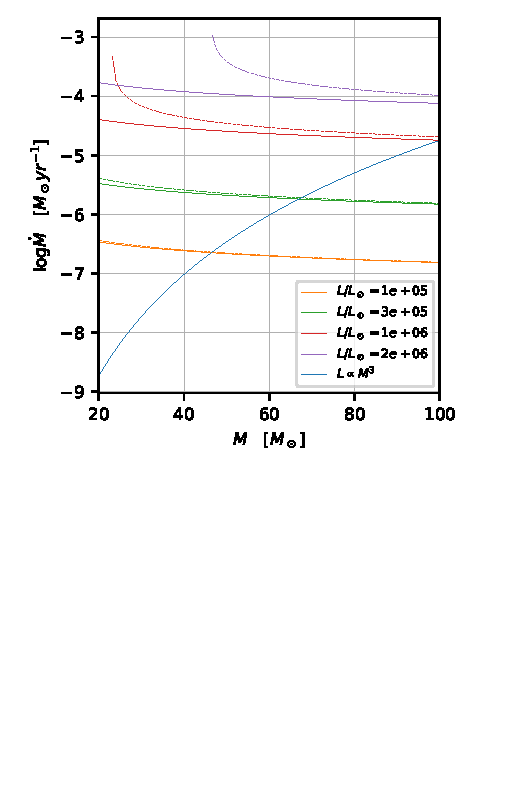
\includegraphics{hw1problem3fig1.pdf}
    \caption{Plot shows the mass loss rate due to winds in hot luminous stars using the equation \ref{eq:massLossRate}. The solid lines are when we are neglecting radiation pressure and the dash lines are with radiation pressure. }
    \label{fig:problem3Fig}
\end{figure}


%==============================================================
\subsection{}
\textbf{Now consider the effects of radiation pressure, by using
\begin{equation}
    \Gamma_e = \frac{\kappa L}{4\pi c GM},
\end{equation}
with all quantities in cgs units, and using the electron scattering opacity for the winds of hot stars with $\kappa = 0.3$ \si{\centi\meter\per\g}.
What is the effect on the mass loss rates?}

Figure \ref{fig:problem3Fig} shows the mass loss rate considering the radiation pressure in dash lines. We can see that the mass loss rate still decreases with M but it seem to be exponential which at larger M it tends to the mass loss rate without radiation pressure.



%==============================================================
\clearpage
%==============================================================
\section{}
\textbf{Photon mean free paths are very short except in the outermost
layers of a star.
This means that photons must take a very long time to escape from a star.
To estimate this time, assume that a photon is created at the center of the star and undergoes a series of random walk scatterings until it reaches the surface.
The mean free path associated with each scattering is $\lambda_{phot} = (n_e\sigma_e)^{-1}$, where $\sigma_e$ is the Thomson scattering cross section $\sigma_e \approx 0.7 \times 10^{-24}$ \si{\square\centi\meter}. 
Assume constant density and $\lambda_{phot}$.}
%==============================================================
\subsection{}
\textbf{Using 1-D random walk arguments, show that $L\approx R^2 / \lambda_{ph}$ is the mean total distance a photon travels if it starts its scattering career at the stellar center and eventually ends up at the surface at $R$.}

Using random walk arguments, we have that the average distance after N steps is equal to
\begin{equation*}
    \frac{R}{\lambda_{phot}}\approx\sqrt{N}
\end{equation*}
and the total distance travelled is 
\begin{equation*}
    L \approx N \lambda_{phot} = \frac{R^2}{\lambda_{phot}^2}\lambda_{phot}=\frac{R^2}{\lambda_{phot}}
\end{equation*}

%==============================================================
\subsection{}
\textbf{Since the photons travel at the speed of light, $c$, find the time, $t$, required for the photon to travel from the stellar center to the surface at $R$.}

We know that the velocity is equal to the distance over time so we can find that the time is
\begin{equation*}
    t = \frac{L}{c} = \frac{R^2}{\lambda_{phot}c} = \frac{R^2n_e\sigma_e}{c}
\end{equation*}
 where $v=c$ for the photons.

%==============================================================
\subsection{}
\textbf{Give a quantitative estimate for $t$, in units of years, for a star of mass $M/M_odot$ and radius $R/R_odot$. Assume solar composition.}

We know that 
\begin{equation}
    n_e = \frac{\rho N_A}{\mu_e} = \frac{\rho N_A (1+X)}{2}=\frac{3MN_A(1+X)}{8\pi R^3}
\end{equation}
where $\mu_e = 2/(1+X)$ where X is the mass fraction of the ions and the density, $\rho$, is given by $\rho = 3 M / 4\pi R^3$ from the constant density model.

Then we have that the time is given by
\begin{equation}
    t = \frac{R^2\sigma_e}{c}\frac{\rho N_A (1+X)}{2}=\frac{3MN_A(1+X)}{8\pi R^3}
\end{equation}

Evaluating all constants, converting the mass and radius in solar units and using $X=0.7$ since we are assuming solar composition, then we get that

\begin{equation}
    t = \SI{8.154e10}{\s} = 2585 \frac{M}{M_\odot}\frac{R}{R_\odot}^{-1} \text{yrs}
\end{equation}

%==============================================================
\clearpage
%==============================================================
\section{}
\textbf{Let's look at corrections to Maxwell- \\ Boltzmann statistics due to weak electron degeneracy (assuming a non-relativistic \\case).
Suppose that $\mu/\kappa T$ is still much less than $-1$, but we wish to include some effects of Fermi-Dirac statistics.
In other words, what are the effects due to the $+1$ in the distribution function?}
%==============================================================
\subsection{}
\textbf{If the exponential term in Eq. 3.9 is still large, then you can use the expansion $1/(a + 1) \approx (1 - 1/a)/a$ to first order in $a$. Assume that $\mu/\kappa T$ is still given by
\begin{equation}
    e^{\mu/\kappa T} = \frac{n_0 h^3}{2(2\pi m_e \kappa T)^{3/2}} \equiv K
    \label{eq:bigK}
\end{equation}
where $n_0$ is the electron number density in the pure Maxwell-Boltzmann limit.
Show that the number density $n$ for weak degeneracy is
\begin{equation}
    n=n_0\left[1-2^{-3/2}K\right]
\end{equation}}

Equation 3.9 from HKT is
\begin{equation*}
    n(p)=\frac{1}{h^2}\Sum_j\frac{g_j}{\exp{-\mu - \epsilon_j + \epsilon(p)}}
\end{equation*}

For this case we can use $g=2$ for fermions, $\epsilon=0$ since we are assuming there's only one energy level, and $\epsilon(p)=p^2/2m$ considering the non-relativistic case. Then
\begin{equation*}
    n(p) = \frac{2}{h^3}\frac{1}{\exp{-\mu/\kappa T}\exp{p^2/2m\kappa T}}
\end{equation*}

Using the expansion $1/(a + 1) \approx (1 - 1/a)/a$ to first order in $a$ and the relation \ref{eq:bigK}, we have that
\begin{equation}
    n(p) = \frac{2K}{h^3}\left(e^{p^2/2m\kappa T}-Ke^{p^2/m\kappa T}\right)
\end{equation}

Then, the number density is given by
\begin{align*}
    n = 4\pi \int_p p^2 n(p) dp\\
    n =  \frac{8\pi K}{h^3}\int_p p^2\left(e^{p^2/2m\kappa T}-Ke^{p^2/m\kappa T}\right)dp\\
\end{align*}
We can note that we have two terms that are similar to $x^n e^{x^{-2}}$ which immediately calls for the use of gamma functions.
For the first integral, we use the following transformation
\begin{align*}
    x = p/\sqrt{2m\kappa T}\\
    dx = dp / \sqrt{2m\kappa T}\\
\end{align*}
and for the second integral, we use
\begin{align*}
    x = p/\sqrt{m\kappa T}\\
    dx = dp / \sqrt{m\kappa T}\\
\end{align*}

Substituting on $n$, we get
\begin{align*}
    n &= \frac{8\pi K}{h^3}\left[(2m\kappa T)^{3/2}\int_0^\infty x^2 e^{x^{-2}} dx \\ 
    &\qquad - K(m\kappa T)^{3/2}\int_0^\infty x^2 e^{x^{-2}} dx \right]\\
    n &= \frac{8\pi K(m\kappa T)^{3/2}}{h^3}\left[2^{3/2}\frac{\sqrt{\pi}}{4}- K\frac{\sqrt{\pi}}{4}\right]\\
    n &= \frac{8\pi(m\kappa T)^{3/2}}{h^3}\left(\frac{n_0 h^3}{2(2\pi m_e \kappa T)^{3/2}}\right)\left[2^{3/2}-K\right]\\
    n &= n_0\left[1 - 2^{-3/2}K\right]
\end{align*}

%==============================================================
\subsection{}
\textbf{Show that the new pressure is
\begin{equation}
    P = n_0\kappa T \left[1-2^{-5/2}K\right]
\end{equation}}

Using the same value of $n(p)$, $v=p/m$ and the same substitution of gamma function we can find the the pressure is
\begin{align*}
    P &= \frac{4\pi}{3m}\int_p p^4 n(p) dp\\
    &= \frac{4\pi}{3m}\int_p p^4 \frac{2K}{h^3}\left(e^{p^2/2m\kappa T}-Ke^{p^2/m\kappa T}\right) dp\\
    &= \frac{8\pi K(m\kappa T)^{2/3}}{3h^3m}\left[2^{5/3}\int_0^\infty x^4 e^{x^{-2}} dx - K\int_0^\infty x^4 e^{x^{-2}} dx\right]\\
    &= \frac{8\pi(m\kappa T)^{2/3}}{3h^3m}\left(\frac{n_0 h^3}{2(2\pi m_e \kappa T)^{3/2}}\right)\left[2^{5/2}-K\right]\\
    &= n_0\kappa T \left[1-2^{-5/2}K\right]
\end{align*}


%==============================================================
\subsection{}
\textbf{In this case of weak degeneracy, what is $P(n)/P_{id}(n)$ to the lowest order in $K$, where $P_{id}(n) = n\kappa T$ is the pressure that an ideal gas of density $n$ would have?
Have a brief discussion of the meaning of the result.}

Substituting the $n$ that we found previously into the equation of an ideal gas, we get 
\begin{equation*}
    P_{id}(n) = n_0\kappa T \left[1-2^{-3/2}K\right]
\end{equation*}
 Then the ratio is
\begin{align*}
    \frac{P(n)}{P_{id}(n)} &= \frac{n_0\kappa T \left[1-2^{-5/2}K\right]}{n_0\kappa T \left[1-2^{-3/2}K\right]}\\
    &= \frac{\left[1-2^{-5/2}K\right]}{\left[1-2^{-3/2}K\right]}.
\end{align*}

This tell us that the pressure considering a weak degeneracy is bigger than that from an ideal gas. We can also note that there will be a discontinuity if $K=2^{3/2}$ and it will be zero if $K=2^{5/2}$. 



% % %\include{name} %name without extension. insert in new page

% \newpage %continues on next column
%\clearpage %continues on next page

% %%%%%%%%%%%%%%%%%%%%%%%%%%%%%%%%%%%%%%%%%%%%%%%%%%%%%%%%%%%%%%%%%%%%%%%%%
%%%%%%%%%%%%%%%%%%%%%%%%%%%%%%% PROBLEM 1 %%%%%%%%%%%%%%%%%%%%%%%%%%%%%%%
%%%%%%%%%%%%%%%%%%%%%%%%%%%%%%%%%%%%%%%%%%%%%%%%%%%%%%%%%%%%%%%%%%%%%%%%%
\section{}
Practice the variable transformation. Please step-by-step prove Eq. (3.97) in the textbook:
\begin{equation*}
    \Gamma_3 -1 = \frac{P}{\rho T}\frac{\Xi_T}{c_V},
\end{equation*}
where $\Gamma_3 - 1 = \left(\frac{\partial\ln T}{\partial\ln\rho}\right)_S$ and $\Xi_T = \left(\frac{\partial\ln P}{\partial\ln T}\right)_V$ and $c_V = T\left(\frac{\partial S}{\partial T}\right)_V$.


%%%%%%%%%%%%%%%%%%%%%%%%%%%%%%%%%%%%%%%%%%%%%%%%%%%%%%%%%%%%%%%%%%%%%%%%%
%%%%%%%%%%%%%%%%%%%%%%%%%%%%%%% PROBLEM 2 %%%%%%%%%%%%%%%%%%%%%%%%%%%%%%%
%%%%%%%%%%%%%%%%%%%%%%%%%%%%%%%%%%%%%%%%%%%%%%%%%%%%%%%%%%%%%%%%%%%%%%%%%
\section{}
\subsection{}
Please first get a numerical expression to estimate the election mean free path $\lambda$ in a white dwarf.

\subsection{}
Then estimate the timescale of the heat transfer via the thermal conduction across a white dwarf, assuming a size of $\approx 0.01R_\odot$, and compare the timescale with that of radiative transfer across the sun. 

\subsection{}
Reproduce $\kappa_{cond}$ of Eq.4.72 in the textbook by \\putting in all the numerical factors left out of the discussion leading up to that equation.



%%%%%%%%%%%%%%%%%%%%%%%%%%%%%%%%%%%%%%%%%%%%%%%%%%%%%%%%%%%%%%%%%%%%%%%%%
%%%%%%%%%%%%%%%%%%%%%%%%%%%%%%% PROBLEM 3 %%%%%%%%%%%%%%%%%%%%%%%%%%%%%%%
%%%%%%%%%%%%%%%%%%%%%%%%%%%%%%%%%%%%%%%%%%%%%%%%%%%%%%%%%%%%%%%%%%%%%%%%%
\section{HSK 5.3}
Characterize the difference of the stellar material from the lab one.
In the Navier-Stokes equation of motion for an incompressible 
fluid (which is consistent with the Boussinesq approximation) we find a drag term $\nu\nabla^2\boldsymbol{w}$, where $\nu$ is the kinematic viscosity having the same units as $\nu_T$, the thermal diffusivity. We replace the Laplacian by $w/l^2$ and amend the equation of motion (5.22 in the textbook) to read
\begin{equation*}
    \frac{dw}{dt}=\frac{(\rho-\rho')}{\rho}g-\frac{\nu}{l^2}w.
\end{equation*}

The additional term always acts to decelerate the parcel. An estimate for $\nu$ is
\begin{equation*}
    \nu \approx \frac{2\times 10^15 T^{5/2}A_{1/2}}{\rho Z^4\ln\Delta_c}\text{cm}^2\text{s}^{-1},
\end{equation*}
where
\begin{equation*}
    \Delta_c \approx 10^4\frac{T^{3/2}}{n_e^{1/2}}
\end{equation*}
and A and Z are the atomic weight and charge of the ions. use this to make an estimate of the Prandtl number
\begin{equation*}
    \boldsymbol{Pr}=\frac{\nu}{\nu_T}
\end{equation*}
for a typical point in the sun. Note that laboratory experiments work around \textbf{Pr}$\approx 1$. What is the main cause for the difference?



%%%%%%%%%%%%%%%%%%%%%%%%%%%%%%%%%%%%%%%%%%%%%%%%%%%%%%%%%%%%%%%%%%%%%%%%%
%%%%%%%%%%%%%%%%%%%%%%%%%%% PROBLEM 4 %%%%%%%%%%%%%%%%%%%%%%%%%%%%%%%%%%%
%%%%%%%%%%%%%%%%%%%%%%%%%%%%%%%%%%%%%%%%%%%%%%%%%%%%%%%%%%%%%%%%%%%%%%%%%
\section{HSK 5.4}
The dimensionless Rayleigh number, \textbf{Ra}, is a measure of how well the driving of convection (as in $\nabla-\nabla_{ad}$ terms) compares to damping processes ($\nu_T$ and $\nu$). It is defined by 
\begin{equation*}
    Ra = \frac{Qg}{\lambda_P}(\nabla-\nabla_{ad})\frac{l^4}{\nu_T\nu}.
\end{equation*}

\subsection{}
Compute a couple of sample values (one in the solar radiative zone and the other in the solar convective zone; e.g., see Fig 5.2 of the textbook). Laboratory experiments have Ra of about $10^11$ or less. Comments?

\subsection{}
Adopt and/or amend the relevant equations in the textbook (i.e., including the viscosity term; see the previous exercise) to show that Ra>1 implies that $w$ and $\delta T$ have exponentially  growing solutions. Laboratory convection usually sets in at about $\textbf{Ra}\approx10^3$.


%%%%%%%%%%%%%%%%%%%%%%%%%%%%%%%%%%%%%%%%%%%%%%%%%%%%%%%%%%%%%%%%%%%%%%%%%
%%%%%%%%%%%%%%%%%%%%%%%%%%%%%%% PROBLEM 5 %%%%%%%%%%%%%%%%%%%%%%%%%%%%%%%
%%%%%%%%%%%%%%%%%%%%%%%%%%%%%%%%%%%%%%%%%%%%%%%%%%%%%%%%%%%%%%%%%%%%%%%%%
\section{6.10 HSK}
Consider the two reactions $X(\alpha,\gamma)Y$ and $Y(\gamma,\alpha)X$, where the second reaction is the photo - disintegration inverse of the first.
The rates for these, in obvious notation, are proportional to $<\sigma\nu>_{\alpha X} n_\alpha n_X$ and $\lambda_{\gamma Y} n_Y$. 
Assume that the two reactions are in equilibrium during silicon burning so that 
\begin{equation*}
    X+\alpha\leftrightarrow{} Y+\gamma
\end{equation*}
where the reactions proceed equally rapidly in both directions.
Therefore, the Saha equation can be used to find $\lambda_{\gamma Y}$ (which is notoriously difficult to find experimentally).
Please prove that
\begin{equation}
    \lambda_{\gamma Y} = <\sigma\nu>_{\alpha X}\frac{g_\alpha g_X}{g_Y}\left(\frac{2\pi m_\alpha \kappa T}{h^3}\right)^{3/2}e^{-Q/\kappa T},
\end{equation}
where Q is the Q-value for $X(\alpha,\gamma)Y$, $m_\alpha$ is the mass of $\alpha$ and is much less than the mass of X, and $gs$ are the statistical weights.
For the $^{24}\text{Mg}(\alpha,\gamma)^{28}\text{Si}$ reaction the binding energies per nucleon for $\alpha$,$^{24}\text{Mg}$, and $^{28}\text{Si}$ are, respectively, 7.074, 8.26, and 8.447 MeV.
What is Q?
What kind of temperatures would this imply for equilibrium?
(This is a bit of a phony because at high temperatures excited states may be populated and these can partake in the reaction.)




% \newpage

\section{}
Suppose that a star is made of ideal gas, is dominated by radiative heat transfer, and is in hydrostatic equilibrium. Furthermore, the specific (per unit mass) energy generation, mean molecular weight, and opacity are the same throughout this star.
Neglecting radiation pressure, please show that the star is a polytrope of index $n = 3$.

\section{}
Use some decent integrator to construct a polytrope with index $n = 3$.
The simplest method is to shoot for a solution. 
Please a) plot $\theta_3$ as a function of $\xi$ and b) calculate $\xi_1$, $-\theta_3^\prime(\xi_1)$, and $\rho_c/\langle\rho\rangle$ and check your results with Table 7.1 in HSK.

\section{}
Estimate the Chandrasekhar's mass of a zero temperature white dwarf, when electrons become extreme relativistic degenerate.
\subsection{}
Show that the equation of state can be expressed as $P=K\rho^{4/3}$ where
\begin{equation}
    K = \frac{1}{4}\left(\frac{8\pi}{3}\right)^{-1/3}\frac{hc}{(m_A\mu_e)^{4/3}}
\end{equation}
in which $\mu_e$ is the mean molecular weight of electrons.

\subsection{}
Show the mass of the white dwarf in this extreme is independent of the radius
R and can be expressed as
\begin{equation}
    M = \frac{1}{4\pi}\left(\frac{3}{2}\right)^{1/2}\left(\frac{hc}{Gm_A^{4/3}}\right)^{3/2}\frac{\xi_1^2\left(-\frac{d\theta_3}{d\xi}\right)_{\xi_1}}{\mu_e^2},
\end{equation}

where the values of $\xi_1$ and $\left(-\frac{d\theta_3}{d\xi}\right)_{\xi_1}$ can be obtained from Table 7.1.

\subsection{}
Finally, show $M=1.44M_\odot\left(\frac{2}{\mu_e}\right)^2$. What is the value of $\mu_e$ for a white dwarf with He, C, O... composition (i.e., $X\sim0)$)?



\section{}
Consider a (fully convective) solar composition ($\mu = 0.61, \mu_e = 1.17$) object at the
star/brown dwarf dividing line. The object can be modeled via a polytrope with
$n = 3/2$.

\subsection{}
Please obtain the central density and temperature as a function of the total
radius (R) and mass (M) of the object in solar units.

\subsection{}
Show how the central temperature depends on the stellar mass when the gas
thermal pressure equals to the electron degeneracy pressure.

\subsection{}
The minimum temperature required to fuse hydrogen is $T_{min}\sim\SI{4e6}{\kelvin}$. Let's
assume that for fusion to occur, the object can't be supported by degeneracy,
i.e., gas pressure must be more important than degeneracy pressure. 
With this condition, what is the transition mass between stars and brown dwarfs?


\section{}
Derive the following equation (see Eq. 7.141 of the textbook, HSK)
\begin{equation}
    T_{eff}\approx 2400(Z/0.02)^{4/51}\mu^{13/51}(M/M_\odot)^{7/51}(L/L_\odot)^{1/102}
\end{equation}
for a completely convective star with $H^{-}$ opacity near the surface (see Eq. 7.126, HSK).




\newpage

%%%%%%%%%%%%%%%%%%%%%%%%%%%%%%%%%%%%%%%%%%%%%%%%%%%%%%%%%%%%%%%
%=====================Add Bibliography=========================
%%%%%%%%%%%%%%%%%%%%%%%%%%%%%%%%%%%%%%%%%%%%%%%%%%%%%%%%%%%%%%%

% \bibliographystyle{plain} % We choose the "plain" reference style
% %plain style sorts the reference list by alphabetical order of the first author’s last name.
% \bibliography{references} % Entries are in the "refs.bib" file

% \clearpage

% %%%%%%%%%%%%%%%%%%%%%%%%%%%%%%%%%%%%%%%%%%%%%%%%%%%%%%%%%%%%%%%
% %=====================Appendix=================================
% %%%%%%%%%%%%%%%%%%%%%%%%%%%%%%%%%%%%%%%%%%%%%%%%%%%%%%%%%%%%%%%
%  \appendix

% \section[]{Python code} 
% \lstset{caption={KingModel.py}, style=Python}
% %\label{sec:CodeHw04p1}
% %\lstset{label={Astro732Hw04P1.py}}
% \lstinputlisting[language=Python]{CodeAndFigures/KingModel.py}

% \newpage

% %\section[]{Python code Problem 3} 
% \lstset{caption={SetupPlots.py}, style=Python}
% \lstinputlisting[language=Python]{CodeAndFigures/SetupPlots.py}

% \newpage

% %\section[]{Python code Problem 4} 
% \lstset{caption={NumericIntegrations.py}, style=Python}
% \lstinputlisting[language=Python]{CodeAndFigures/NumericIntegrations.py}

% \newpage

% %\section[]{Python code Problem 5} 
% \lstset{caption={Astro645HW04p5.py}, style=Python}
% \lstinputlisting[language=Python]{CodeAndFigures/Astro645HW04p5.py}


\end{document}